\chapter{Payload Design Tradeoffs}

\section{Means of Securement}\label{PL:Tradeoffs:Securement}	
	\subsection{UAV Arm Configuration}
		\subsubsection{Parallel Unfolding Arms}
			The team came up with two ideas for the structure of the UAV, both of which satisfied the compact structural requirements needed for this competition. The first idea was to have the arms of the UAV unfold in a spiral fashion. During the pre-deployment stage, the arms would assume an initial form folding parallel to the four sides of the body of the UAV. Four servos would then be used to rotate the arms outward. 
		
			One benefit of this structure is that the UAV would be more adaptable to different flying environments and possible motor failures. The unfolding process would also be actively controllable. While in the maximized allowed angle, which for the purpose of this competition’s flight would be 90°, the four arms would be held in place with the use of a locking mechanism called limit pin. This locking design would ensure the flight stability and increase the overall structural integrity of the system. 
			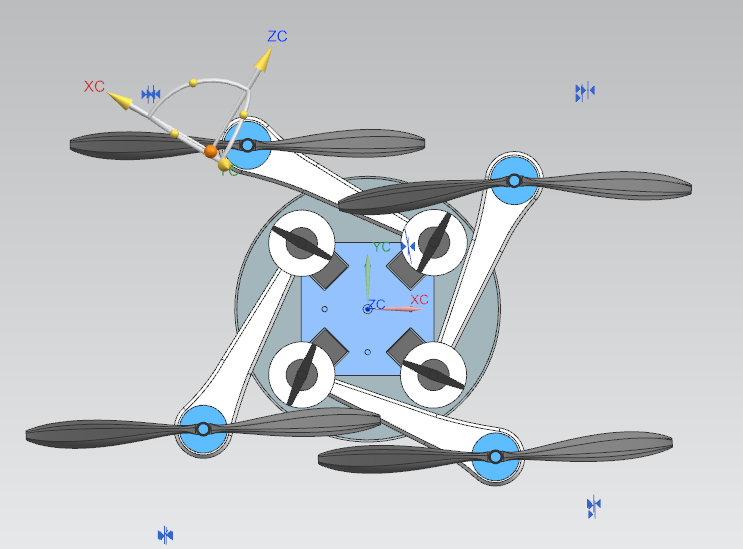
\includegraphics[width = 7cm, height = 7cm]{img/PL/topold.PNG}
			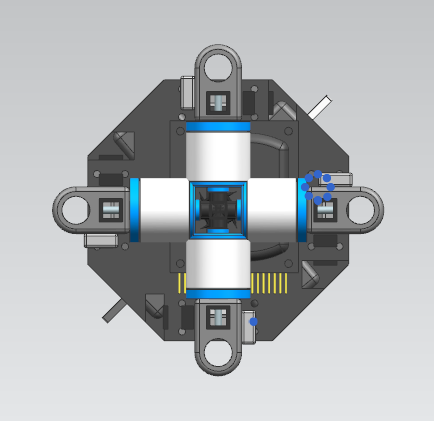
\includegraphics[width = 7cm, height = 7cm]{img/PL/topnew.PNG}
			In spite of being very versatile when facing different circumstances, the foldable arm design had a few shortcomings that ultimately led the team to choose the latter design. As seen in the figure above, the most significant drawback of the side-folding arm structure was that the UAV size would need to be decreased by a considerable margin in order to fit the UAV body and the folded arms inside the body tube. This design would also require a decrease in the length of the arms compared to the upward-folding arm design. This could lead to a decrease in stability during flight. 
		
			Additionally, the pre-selected propeller would also have to decrease in size to accommodate the new dimension. This reduces efficiency and degrades flight time. A foldable design with the use of four servos would also result in a smaller PCB bay, which would lead to a decrease in battery size and therefore negatively affect the potential flight time. The UAV with the vertical folding arm structure can be seen below.
		

		\subsubsection{Vertically Unfolding Arms}
			The top-down unfolding mechanism is the team’s second approach to create a compact UAV that could fit inside the pre-selected body tube dimension. With the mindset of designing a mechanically sound and simple unfolding mechanism, the team decided to place the arms that could be easily deployed through a well established mechanical system. A simpler approach involves certain compromises, but the team decided that the benefits of this design outweigh the potential downsides. 

			This top down approach involves the use of a set of four hinge mechanisms, a set of springs and locking systems. With the lack of an active deployment strategy like the servos mentioned in the above section, the arms have to be deployed mechanically with the assistance of pre-stored potential energies from springs: preloaded strings will push the arms downward with the absence of constraints. One solution the team came up with is the use of four symmetrically placed low-friction aluminum guide rails that serve both as a guiding mechanism for the UAV deployment and as a horizontal constraint for the spring mechanism.
	
	\subsection{Locking Mechanism}
    Once the UAV is free and the arms deploy to the open position, a series of pins are necessary to lock the arms in the proper X4 drone layout.  Once the arms get to a certain orientation,the locking pins will restrict the motion of the arms, locking them in place providing a better flight.  The locking pins on the UAV will operate using the internal tension of PLA to lock the arms in place.  As the arms are released from the guide rails, the pins will push on plastic, and as the plastic bends, and the pins reach the right location, the PLA will snap back in place locking the arms’ position.   


\section{Means of Deployment}\label{PL:Tradeoffs:Deployment}
	The challenge posed to the team regarding the release of the payload is to deploy the UAV in the proper orientation for flight. The UAV requires a fast, consistent, and reliable release mechanism to deploy it from the rocket. During descent, the UAV will be deployed out of the top of the rocket as described below. 

	\subsection{Launch Rails}
		The drone is secured within the rocket with guide rails. The retracted arms are connected to guide rails that hold the drone securely and will guide the drone out of the head of the rocket. The arms fold vertically as shown in the CAD models. Upon release, the drone will slide down the guide rails, out of the head, and the arms will flip open. This process must be controlled to ensure the drone comes out and deploys fully and in the correct orientation. A mechanism will be used to control the drones descent out of the rocket and ensure that the drone is ready before releasing it from the rocket.

	\subsection{Lowering Mechanism}
		To control the speed of the drone exiting the rocket, a lowering mechanism will be used to limit the speed. The mechanism can be either passively controlled through friction or actively controlled through a servo motor. The passive system relies on friction in the winch. 

		One option is for a servo motor to tactically lower the UAV by an exact amount at an exact speed. The UAV can be accelerated and decelerated at the beginning and ending of its descent to ensure it doesn't experience extreme jerk. This will ensure the further safety of the UAV. Since only the descent of the UAV needs to be controlled, the motor does not need to be powerful. The motor can be geared to the speed necessary to deploy the UAV. However, the motor can fail. It requires electronic input and has more points of failure than a passive friction system.
	
		The passive system will eliminate the points of failure that arise from the use of a servo. The winch can be built with a specific resistance to restrict the acceleration of the drone as gravity pulls it out of the rocket. One benefit of this solution is that it will also keep costs down. However, this solution poses a larger threat to the safety of the drone. The drone will accelerate out of the rocket and may be traveling at a high velocity when the limit of the winch is reached. In this case, the drone could experience a large jerk, which could cause damage.The descent will also have less control, resulting in a less consistent deployment.
	
	\subsection{Lowering Mechanism Release System}
		Once the UAV has been deployed outside of the rocket, the line attached to the winch must be disconnected. The team came up with three potential ways to accomplish this. The first option utilizes a sharp cutter attached to the UAV to sever the string. The second option uses a quick-release mechanism attached to the UAV to disconnect the line. Lastly, a nylon string could be attached to a winch and an electric connection could be used to burn through the nylon string. 

		The cutter mechanism would require mechanical components and a motor to execute the operation. The design is simple, but will require care to ensure that the cutter will completely sever the string in all conditions, such as in both the presence and the absence of tension. 
	
		The quick-release mechanism is similar to the cutter mechanism. It will require a motor or similar mechanical source to pull a pin. The advantage of this system is that it does not depend on the line being cut. This also allows the line to be made of almost any material, including options more durable than nylon that do not cut easily. However, the quick-release would need to be designed carefully to ensure that it is not accidentally triggered before intended. The risk of premature triggering of the release is significant, and factors heavily into the team’s consideration of the viability of this option. 
	
		The electric system is a viable option for burning through nylon string. This system has no moving parts, which corresponds to less points of failure. It is the most reliable option. However, it will could longer to burn through the string than it might take to execute the other options. Additionally, this system limits the material for the string to nylon. 
	

	\subsection{Nose Cone Jettison}
		\subsubsection{Previously Proposed Nose Cone Recovery System}
            As described in the proposal, the team will integrate UAV deployment with the nose cone deployment. Once deployed, the UAV will drop the nose cone from a calculated altitude based on the limit of kinetic energy under free fall. For reference, the UAV within the nose cone can be seen in the figure below.

            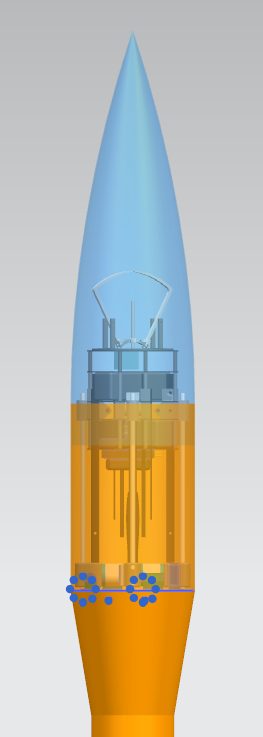
\includegraphics[width = 7cm, height = 7cm]{img/PL/jet.PNG}
        
            This idea has since been re-evaluated following the submission of the proposal. The primary concern with this deployment method is the increase in power consumption due to the additional weight being carried by the UAV, which will have a negative impact on overall flight time. Additionally, the solenoids used to detach the nose cone from the vehicle will not be used for the remainder of the mission, rendering them redundant from that point on. The team’s secondary concern is the risk of a free falling component. The team had to consider the potential for a faulty tethering mechanism of the nose cone to the UAV. In this case, the landing of the nose cone would be ballistic, meaning a hazardous descent. Because of this, a design review of the deployment method was addressed to ensure safe simultaneous deployment of the nose cone and UAV payload. 

		\subsubsection{Redesigned Nose Cone Recovery System}
        In order to ensure safe descent of the nose cone and minimize the risk of it interfering with UAV deployment, the team decided to design a parachute recovery system. The recovery system will consist of a 12” parachute from Fruity Chute. The parachute is made out of Ripstop Nylon with a drag coefficient of 0.8. A Jolly-Logic Chute Release will be used to ensure that the nose cone does not drift too far from the launch site.

        Most commercial parachute release mechanisms for ameteur rockets utilize black powder charges to separate the airframes and deploy the recovery system. However, this is not an option when deploying the nose cone recovery system as it poses too much of a threat to the UAV payload. Black powder is a highly explosive material and introduces more risks to the team, the rocket, and its contents. Instead, the team has opted to implement an exhaustless Tinder Rocketry CO\textsubscript{2} canister deployment system. With this method, the payload bay is not exposed to hot gasses emitted from an explosive charge. Ejection via a 16 g CO\textsubscript{2} canister has been deemed a safer, more reliable, and less detrimental way to deploy the rocket components. 
        
        The CO\textsubscript{2} ejection system will be activated by a commercial altimeter housed in the payload bay. The altimeter will trigger an e-match at 700 ft that ignites a small (0.15 g) black powder charge. This height should provide an adequate amount of time for the UAV system to deploy and actuate before cutting its tether under the 400 ft ceiling requirement. The housing of the CO\textsubscript{2} system is equipped with O-rings, completely sealing the charges in the chamber and effectively containing the pyro exhaust. The combustion contained is immediately cooled due to the CO\textsubscript{2} released. Because of this, the system can be mounted in the same compartment as the payload without risk of damaging the payload and any sensitive avionics. 
        
        The CO\textsubscript{2} deployment system will be located in the nose cone itself, however the commercial altimeter used to trigger the deployment system will be located on the lower bulkhead of the payload bay. In order to connect the pyro charge that will trigger the CO\textsubscript{2} system to the altimeter, a two pin JST connector. This JST connector is intended to be pulled apart at the moment of nose cone ejection by the force of the ejection itself. The use of this connector ensures a reliable electrical connection between the altimeter and the CO\textsubscript{2} system up until nose cone ejection. Tug testing will be conducted to ensure the connectors will reliably separate. 

        The size of the canister needed can be determined based on a sizing chart from Tinder Rocketry. However, given the complex geometry of the upper airframe, the team decided to perform volumetric calculations to determine the amount of CO\textsubscript{2} needed to pressurize the chamber and separate the nose cone. The nose cone itself has an ogive shape with dimensions shown in CHART REFERENCE.  Based on this information, volume calculations of the nose cone were done by integrating the tangent ogive formula.

        \begin{subequations}\label{parachute}
            \begin{equation}
                \rho = \frac{R^2 + L^2}{2 R}
            \end{equation}
            \begin{equation}
                y = \sqrt{\rho^2 - (L - x)^2} + R - \rho
            \end{equation}
            \begin{equation}
                V = \pi \int_{0}^{L} y^2 dx
            \end{equation}
        \end{subequations}
\section{Payload Structures}\label{PL:Tradeoffs:Structures}
	\subsection{Landing Leg Design}
		In order to create a safe and gentle touch down for the UAV before initiating task-specific maneuvers, a set of landing systems are needed. The team came up with two different approaches that result in two dissimilar ways to store the landing legs and each of which has its stability factor which will be analyzed in the following paragraphs alongside with risk analyses.
		\subsubsection{Retractable Landing Mechanism}
			The first landing mechanism uses the concept of a parallel four bar linkage. This format allows the legs to fold up as the arms of the drone fold up. This design allows the team to maximize the utility of space inside the body tube. The parallel four bar linkage system allows the legs to be vertical at all times, including the pre-deployment period when the arms are folded in the vertical direction. This unfolding process can be seen in the images below.

            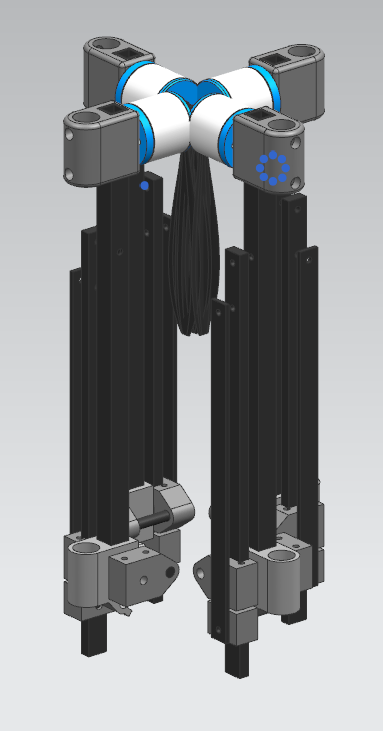
\includegraphics[width = 7cm, height = 7cm]{img/PL/folded.PNG}
            Folded arm configuration

            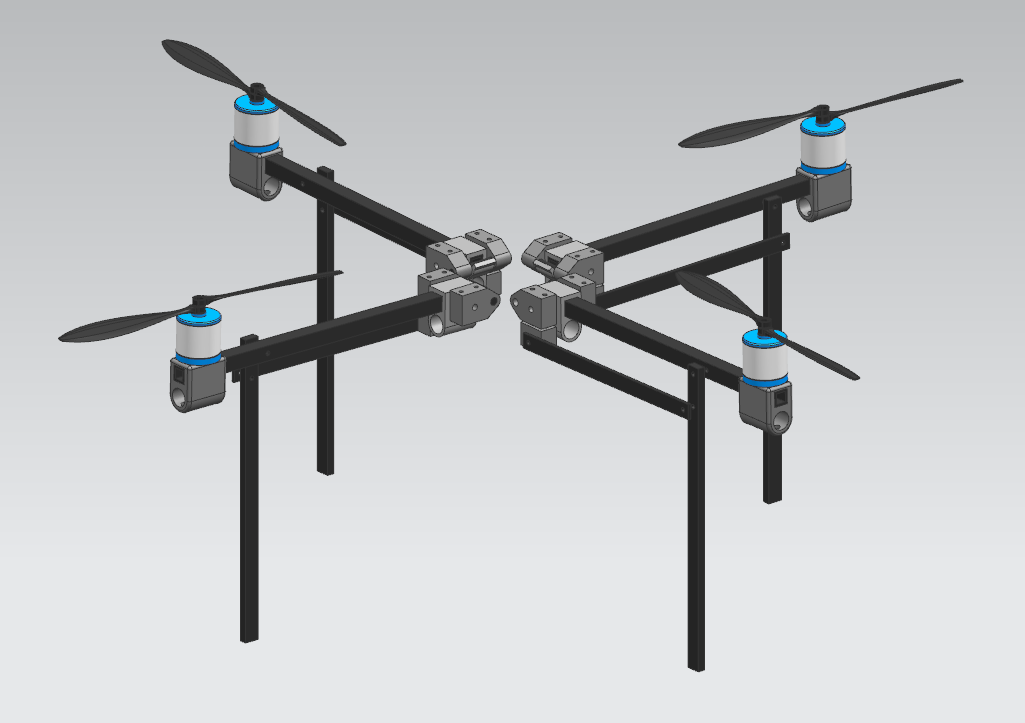
\includegraphics[width = 7cm, height = 7cm]{img/PL/unfolded.PNG}
            Unfolded arm configuration

			The sets of retractable landing mechanisms will be sized based on the overall vertical length of the IRMA system while taking the stability factor into consideration. In order to prevent the chance of IRMA system directly making unintended contact with the ground and suffer damage, the final separation distance between the legs is 281 mm which is more than three times that of the static legs which allows the UAV to have its desired stability upon landing. The team also decided to use twill weave carbon fiber as the material for landing legs due to its high tensile strength under extreme conditions and its lightweight. 

            The maximum thickness of the carbon fiber legs is also selected so that its entirety is contained within the 6” boundary of the body tube. The joints’ mobility factor will also be taken into consideration and the team will conduct multiple testings to ensure its ease at retracting in various different conditions.


		\subsubsection{Static Landing Mechanism}
            The pros and cons of a more conventional set of “static” legs were also analyzed. The static legs will have a length of 114.3 mm made of 3D printed High-Density Polyethylene and will be installed with a set of four cone shaped landing pads at the root of the legs. The landing pads will have an optimal curvature with a radius of 5 mm and with the implementation of metal ball bearings, they will be able to rotate in all directions and adjust to all kinds of terrains. The team estimated the UAV mass with its full payload capacity to be 2.5 kg. Therefore, to have an overall safety factor of 300 percent, every connecting joint of the UAV shall be able to withstand an omnidirectional force of 18.375 N. 

            A design based on the use of static landing legs will produce a few dimensional constraints due to the size of the payload bay. In the current design, the avionics section occupies a planer area of 8665 mm*mm. This provides a total separation distance of 93.08 mm between the static arms. Although this dimension seemed to provide enough stability for any commercial purpose UAVs, it does not satisfy the stability factor for the purpose of our mission. In comparison to the distance mentioned in the above section provided by the unfolding landing legs, this design provides a distance that is more than three times less which increases the possibility of induced tipping. 
            
            Another downside to the static leg design is that in order for them to be safely stored within the rocket, they have to be placed within the nose cone alongside with the IRMA system. Not only does this design take up a good portion of the very limited space the payload has in the rocket, but also induces possible damage during ascent due to the rocket’s vibrations.  
              

	\subsection{Ice Retrieval and Mobility Agent}
		\subsubsection{Pin Joint Mechanism}
			The goal of the payload is to retrieve ten milliliters of ice and move the ice from one bucket to another. To achieve this, the team decided to construct a claw-like mechanism to scoop the ice from underneath the drone, close the claw, and drop the ice in the bucket at the destination. The design has a servo rotate a bolt with a nut without moving the bolt vertically. The nut then moves with respect to the bolt, thus opening the claw as the nut moves down. To close the claw, the nut moves up and the lever arm becomes horizontal, thus pushing the top of claw arm outward. The bottom of the claw will have a slanted shape to easier scoop ice pieces and lower the risk of pushing the ice pieces outwards. 

			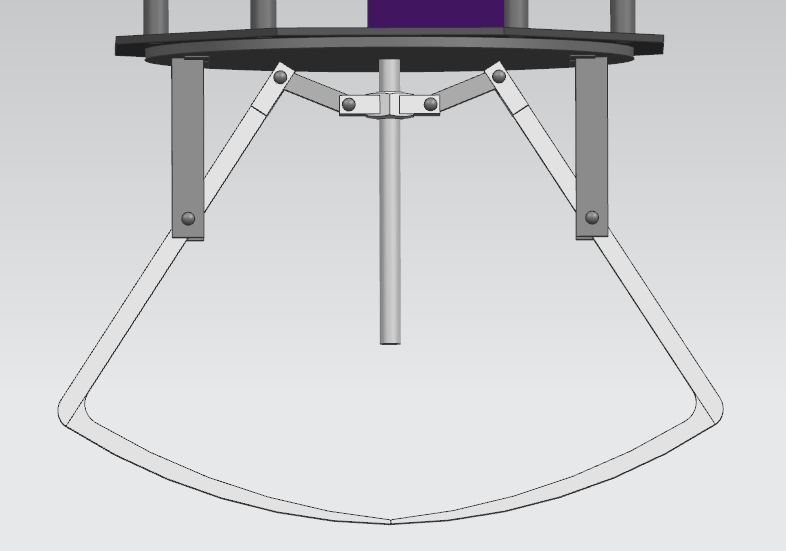
\includegraphics[width = 7cm, height = 7cm]{img/PL/pin1.PNG}

		\subsubsection{Sliding Pin Mechanism}
			Another design the team is considering for the Ice Retrieval and Mobility Agent is a sliding pin mechanism. The sliding pin mechanism relies on the same movement of a nut sliding down a bolt to open and close the claws, but instead of a pin, it has slots that force the scooping mechanism to move out and in. To secure the scooping mechanism to the drone, two rods with pins at each end will be secured to the drone. The pin will connect the scooping mechanism to the rods and thus the drone. The figure shows the sliding pin mechanism closed (left) and open when the pin is near the top of the slot (right). 

			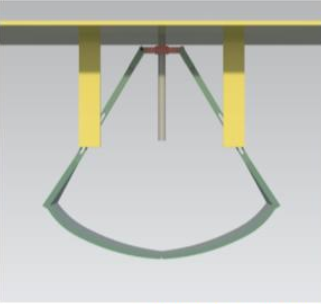
\includegraphics[width = 7cm, height = 7cm]{img/PL/slide2.PNG}
			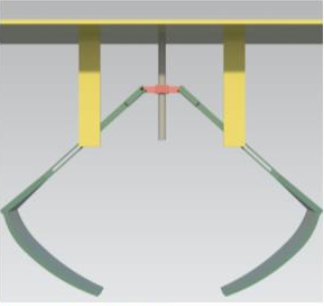
\includegraphics[width = 7cm, height = 7cm]{img/PL/slide1.PNG}

		\subsubsection{Wormgear Mechanism}
			The third consideration was a design that operated using a worm gear to control the claw motion. A fixed position, vertically-oriented worm gear would be rotated using a servo. On either side of the worm gear are conventional round gears that naturally contra-rotate with respect to each other due to the radial symmetry of the worm gear action. The solid claw arms directly mount to their respective round gears, so that as the gears rotate, the arms swing open or closed about the same rotation axis as seen in the figure below. The rotation axes are provided by pin joints located on vertical support bars connected to the underside of the drone(not shown).

			It is easy to obtain the critical components of the design since worm gear packages are readily available in a wide range of sizes. Also, the design is very simplistic and easy to build. A major factor against the worm gear design is the cost of materials. Worm gears are harder to manufacture than round gears, and thus cost more. We decided against spending a large sum of money for a single mechanism. A critical aspect in the structural soundness of the design was identified in the region where the claw arms attached to the gears. The forces acting on the gears would have to be accounted for, and reinforcement of the region may offset the simplicity advantage of the overall design.
			
			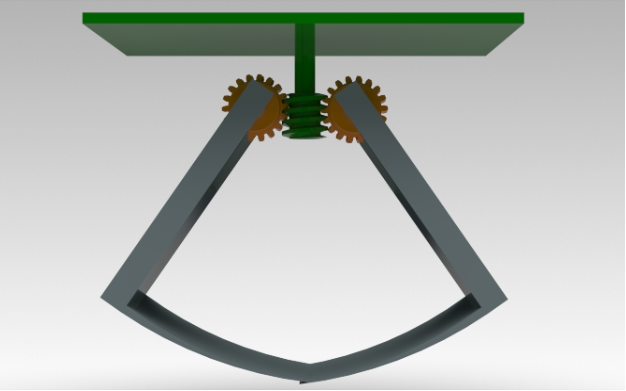
\includegraphics[width = 7cm, height = 7cm]{img/PL/worm2.PNG}
			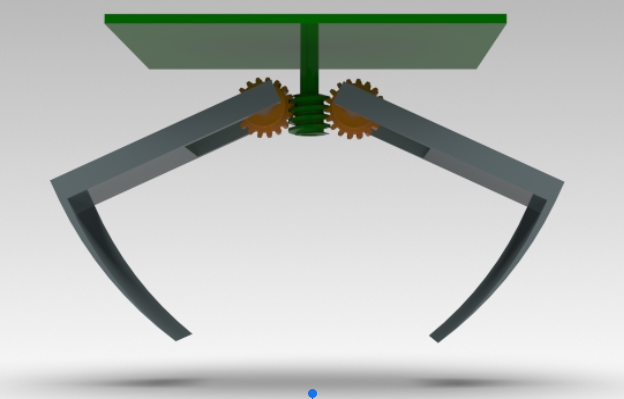
\includegraphics[width = 7cm, height = 7cm]{img/PL/worm1.PNG}
			

\section{Payload Avionics}\label{PL:Tradeoffs:Avionics}
	\subsection{Computer Vision}
		\subsubsection{Algorithmic Approach}
        The team is considering an algorithmic approach to implement the computer vision using OpenCV libraries for Python. Algorithmic computer vision is a novel technique used to quantify elements of visual perception. This provides a systematic and robust way of fabricating automatic synthesis of specialized recognition schemes. Selected features will be used for recognition and localization of particular objects in a given scene. 

        The computer vision will be implemented using the OpenCV library for Python. OpenCV provides a core module that contains a lot of built-in primitives to handle operations related to image processing. These include steps for isolating objects of a given target, determining the size of an object (in pixels), and calculating the centroid of an object. These structures are already optimized for speed and memory. 
        
        The retrieval tracking script can be broken into three parts. The first is the handling of image acquisition, the frame buffer, and the output module to the controller allocation. The basic components of the digital image processing system is given below. 

        The Raspberry Pi’s camera will be utilized to capture a digital image. From here, the image is quantified through a series of algorithmic and logic operations applied at the lowest level of abstraction. This is done to improve image data that suppresses unwanted distortions or enhances image features important for success of future image processing. The input data is then converted to a suitable form for computer processing. The image is partitioned into multiple segments. This process simplifies and changes the representation of the image into constituent parts or objects for easier analysis.

        This input data will be stored as color data memory as the frame buffer. Color can be defined as an ordered triple of the color components in the Red-Green-Blue color space. Each color is represented as an integer in the range [0, 255] requiring 8 bits of memory. This is the standard process for image processing representation of colors in computer vision. From here, desired features are extracted to allow quantitative differentiation of features and objects.

        Arithmetic operations will be applied to describe the retrieval site for the UAV based on basic features that define color. Brightness will be described as a logarithmic function to the light intensity which can be analyzed as a discrete set of brightness points regardless of color. The predominant spectral color in the light is then analyzed as the hue to show the different color attributes. Additionally, saturation will be modeled to indicate the spectral purity of the color in the light. A variety of mathematical methods will then be applied to identify points of discontinuities based on sharp contrasts in the digital image. These discontinuities will identify the retrieval site. Once features have been analyzed, the image processing system will then assign a label to the object based on the information provided by the descriptors. The final process is assigning meaning to the ensemble of recognized objects for controller allocation. 


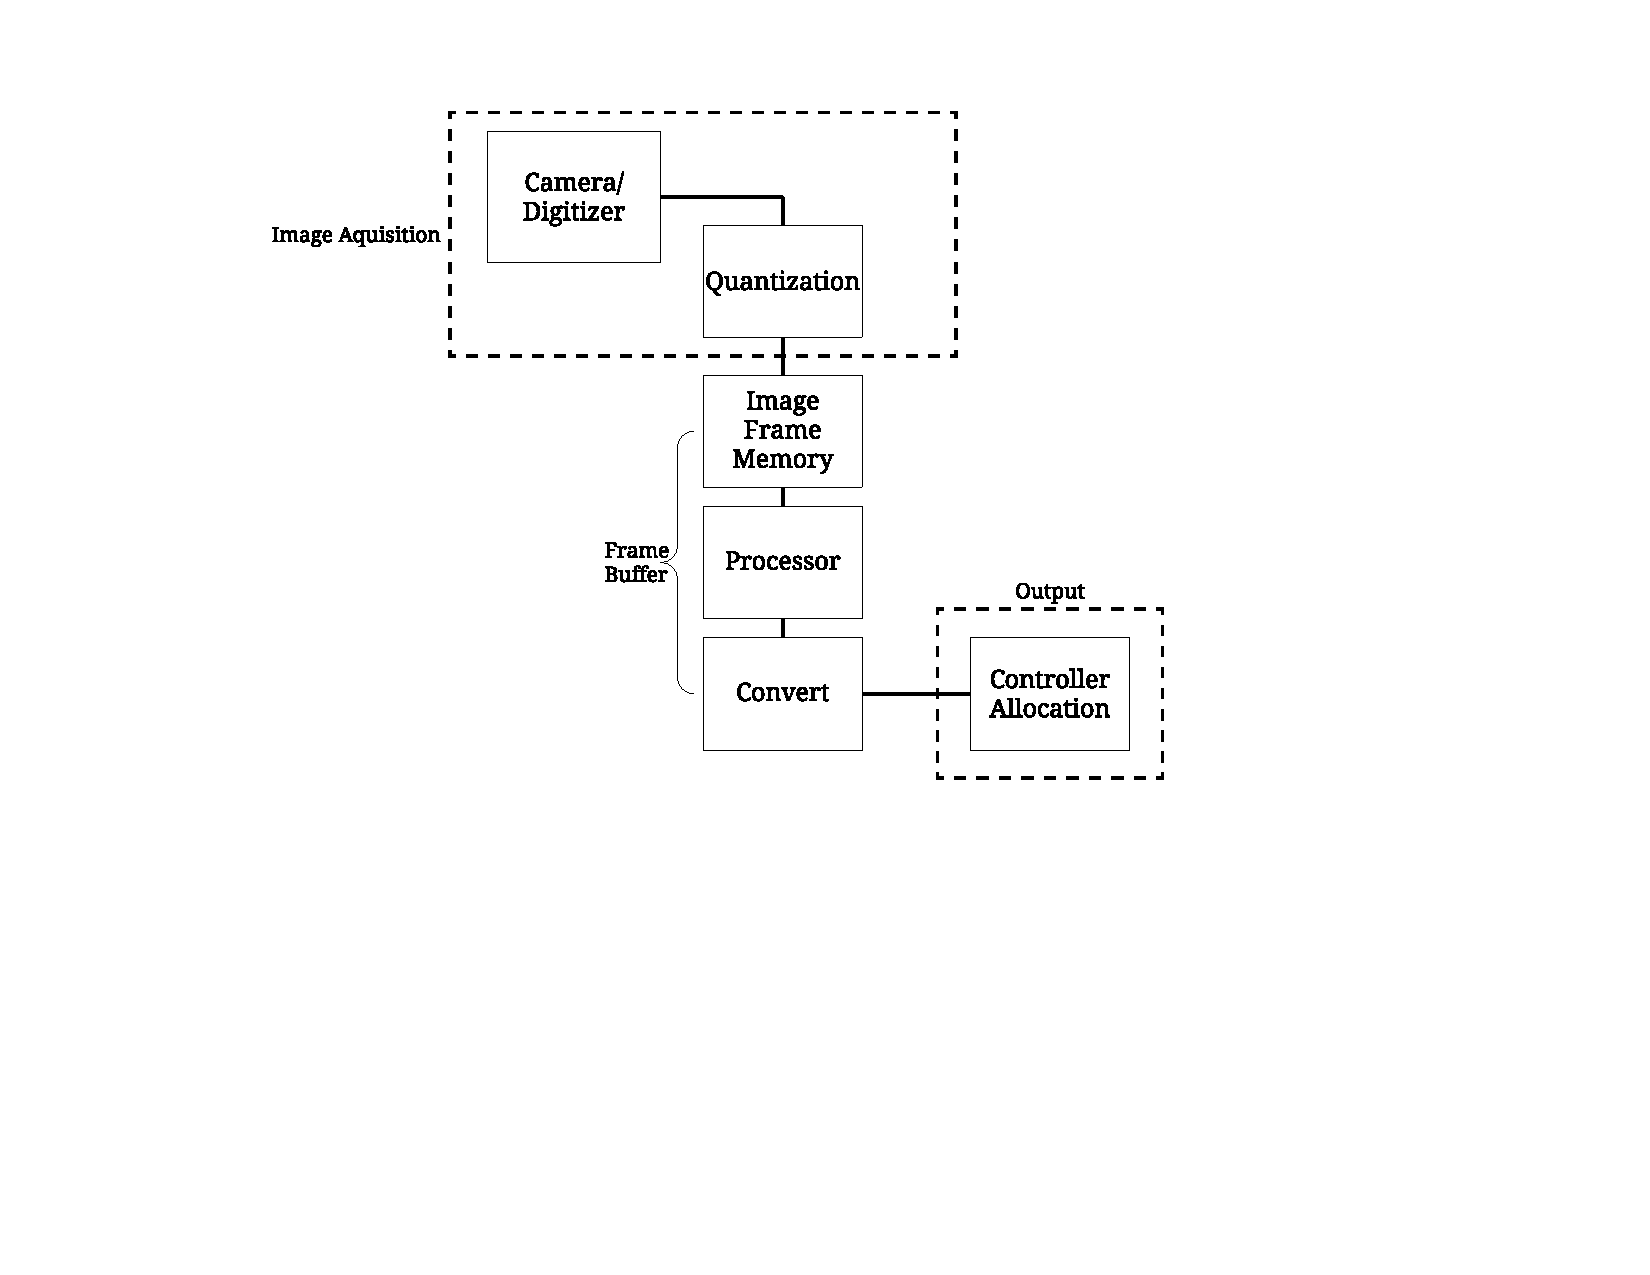
\includegraphics[width = 10cm, height = 10cm]{img/PL/digital.pdf}

		\subsubsection{Deep Learning Approach}
			The deep learning approach to using computer vision on the drone is to utilize neural networks. Neural networks can be used to detect and classify objects; they are used in various emerging technologies, such as self-driving cars and automatic facial recognition. 
			Neural networks function by consecutively modeling small pieces of information and then combining them to form templates, and then finally weighing inputs with the templates to create a final prediction.
		
			During a training process, neural networks utilize algorithms that automatically find patterns in objects by evaluating external features of the object, such as color and structure, to divide objects into different classes. The process then updates weights, which correlate to the strength of association from an input image to the prediction, for the model and improves the performance every iteration. By doing so, it results in minimal error when evaluating the input images.
		
			For the competition, the process would require the team to feed the neural network images similar to that of the excavation area to “train” it to recognize what the excavation area would look like.These images would have labels and tags on them that identify each object. The neural network would analyze features such as the color of the boundary of the excavation area, and then update weights for the excavation area class. The same thing can be done with images of the “ice” sample that needs to be retrieved. Images with different amounts of ice can be input into the neural network to teach it the difference between areas with a high or low amount of ice concentration. Doing so would aid the drone in deciding the specific area it should retrieve the ice from.
		
			Neural networks have specific benefits and setbacks that need to be considered before choosing an approach to employ for computer vision. One useful benefit is that if the neural network is trained correctly, it can be extremely fast, and would be able to detect different objects accurately and reliably. On the other hand, a major setback to using a deep learning approach is the immense training time needed. The number of images needed to train the neural network to an adequate level is unknown, but could range from 1,000 to 100,000 comparison images, based on previous implementations.

 \begin{table}[]
                \label{computer vision}
                {\footnotesize
                \caption{Risk Matrix for Computer Vision}
                \centering
                \begin{tabularx}{\linewidth}{XXXlXl}
                \toprule
                \textbf{Risk}                                            & \textbf{Cause}                                                                                                                 & \textbf{Impact}                                                                                                                           & \textbf{RBM}  & \textbf{Mitigation}                                                                                                                                                                                     & \textbf{RWM} \\
                \midrule
                Algorithm does not recognize excavation site & 1) Incorrect implementation of logic in algorithm relating to classification of excavation sites \newline 2) Not enough images classifying excavation sites are fed to train the neural network to a reliable state & UAV does not navigate to excavation site with complete accuracy & \cellcolor{red!25} 2A & 1) Conduct extensive testing to ensure that algorithm recognizes excavation site accurately and reliably \newline 2) Algorithm reverts to GPS based positioning to navigate to excavation area if excavation site is not recognized. & \cellcolor{green!25} 3D \\
                Algorithm falsely detects an excavation area & 1) Incorrect implementation of logic in algorithm relating to differentiation between excavation sites \newline 2) Not enough images are fed to train the neural network reliably & UAV fails to navigate to correct excavation site and flies to wrong site instead & \cellcolor{red!25} 2A & 1) Conduct extensive testing to ensure that algorithm recognizes excavation site accurately and reliably without detecting incorrect sites \newline 2) Algorithm is manually reverted to GPS based positioning to navigate to correct excavation area & \cellcolor{orange!25} 3C \\
                Algorithm does not run at all or runs slowly & 1) Flight computer is disconnected from power source \newline 2) Algorithm is inefficient through redundant computation or overuse of storage & UAV is not able to recognize and navigate to the excavation site & \cellcolor{orange!25} 2C & 1) Ensure UAV is connected securely to power source, and is able to stay secured during flight \newline 2) Test algorithm during flight to ensure it does not overuse processing power or storage & \cellcolor{green!25} 2E \\
                Algorithm causes Raspberry Pi to malfunction & 1) Algorithm encounters stimulus outside of its training bounds \newline 2) Inaccurate data is fed to algorithm during flight. & UAV malfunctions and loses ability to stay aloft & \cellcolor{red!25} 1C & 1) Conduct extensive testing and identify when Raspberry Pi malfunctions \newline 2) Identify edge cases that may cause malfunctions and account for them in algorithmic approach \newline 3) Catch errors in runtime and deal with accordingly to maintain mission feasibility & \cellcolor{green!25} 1E \\
                \bottomrule
                \end{tabularx}
                }
            \end{table}
	    
	\subsection{Flight Controller}
		From the multitude of different flight controllers available that would suit the mission parameters, the team was able to narrow the list down to 3 choices. These flight controllers, the ArduPilot APM, the Pixhawk 4 and the Navio2, are all widely used by the UAV community. The team identified the factors that were most pertinent to the mission and weighted them by their importance. Ultimately, the flight controller in tandem with its companion computer would require the adequate processing power for the computer vision system and a high degree of reliability, which often varies depending upon software or physical design.

		\subsubsection{ArduPilot}
			The ArduPilot APM, although revolutionary on its initial release, has several downfalls. The most severe of which is its lackluster 8-bit processor. It consists of two components, the main processor board and the IMU shield that can be attached on top. The APM’s framework is based on that of the Arduino Mega and is capable of tasks such as autopilot, autonomous stabilization and way-point based navigation.

		\subsubsection{Pixhawk}
			The Pixhawk is also a renowned flight controller. It contains a much more powerful 32-bit processor and a built-in IMU + Barometer. One of the benefits of the Pixhawk is its ability to interface with a companion computer, such as a Raspberry Pi. A setup like this would be ideal for the high computing power a computer vision navigation system would require.

		\subsubsection{Navio2}
			The Navio2 is slightly different from the Pixhawk and ArduPilot APM; it requires a Raspberry Pi to function. The Navio2 itself is just a shield containing high resolution sensors, a UART interface and a GNSS receiver that fits onto a Raspberry Pi. This combined system coalesces to become the flight controller. A set up like this removes the need to carry an extra companion computer in addition to the flight controller because the flight controller system itself has a high power, 64-bit, 1.5 GHz processor on the Raspberry Pi which can handle the processing needs for the computer vision system.

		\begin{table}[H]
			\centering
			\caption{Flight Controller Fact Sheet}
			\label{tab: flight controller}
			\begin{tabularx}{1\linewidth}{X X X X}
				\toprule
				Factor & ArduPilot & Pixhawk + RaspberryPi & Navio2 \\
			   \midrule
			   	Size (mm) & 70.5 x 45 x 10 & 44 x 84 x 12 & 55 x 65 \\
				Mass (g) & 31.0 & 15.8 & 23.0 \\
				Ease of Integration & 8-bit processor requires aid of companion \mbox{computer} and several peripheral sensors & Requires configuration of linux files to set up UART bridge & Very easy due to extensively tested integration procedures\\
				Power \newline consumption (W) & 0.5 & 3.6 & 2.79 \\
				Reliability & No fall back option & Failures can occur in UART connection & Reliable integration due to 3rd-party product \mbox{design} \\
				\bottomrule
			\end{tabularx}
		\end{table}
 \begin{table}[H]
            \centering
            \caption{Flight Controller Fact Sheet}
            \label{tab: flight controller}
            \begin{tabularx}{1\linewidth}{X X X X}
                \toprule
                Factor & ArduPilot & Pixhawk + RaspberryPi & Navio2 \\
               \midrule
                Size (mm) & 70.5 x 45 x 10 & 44 x 84 x 12 & 55 x 65 \\
                Mass (g) & 31.0 & 15.8 & 23.0 \\
                Ease of Integration & 8-bit processor requires aid of companion \mbox{computer} and several peripheral sensors & Requires configuration of linux files to set up UART bridge & Very easy due to extensively tested integration procedures\\
                Power \newline consumption (W) & 0.5 & 3.6 & 2.79 \\
                Reliability & No fall back option & Failures can occur in UART connection & Reliable integration due to 3rd-party product \mbox{design} \\
                \bottomrule
            \end{tabularx}
        \end{table}
        \begin{table}[H]
            \label{Flight Controller}
            {\footnotesize
            \caption{Risk Matrix for the Flight Controller}
            \centering
            \begin{tabularx}{\linewidth}{XXXlXl}
            \toprule
            \textbf{Risk}                                            & \textbf{Cause}                                                                                                                 & \textbf{Impact}                                                                                                                           & \textbf{RBM}  & \textbf{Mitigation}                                                                                                                                                                                     & \textbf{RWM} \\
            \midrule
            UART bridge disconnects and stops communication & 1) High vibrations during launch and deployment interfere with physical connection.                                  & Complete loss of UAV control and inability to complete mission.                                                                 & \cellcolor{red!25} 2B  & 1) Mechanically secure physical connections of UART port using adhesives and 3D printed constraints. \newline 2) Surround ports with padding to ensure minimal movement.                               & \cellcolor{orange!25} 2D  \\
            Battery failure leads to loss of power          & 1) High vibrations lead to battery disconnecting from flight controller. \newline 2) LiPo batteries overheat                   & 1) Complete loss of UAV control and inability to complete mission. \newline 2) Permanent damage to UAV structure and peripheral sensors. & \cellcolor{red!25} 2B  & 1) Mechanically secure physical connections of batteries using adhesives and 3D printed constraints. \newline 2) Monitor LiPo batteries carefully during pre-flight charging to prohibit overcharging. & \cellcolor{orange!25} 2D  \\
            Noisy data is fed to control loop.              & Turbulence during flight causes instability for UAV airframe, resulting in control algorithms responding improperly. & 1) Unstable flight results in loss of sample from IRMA. \newline 2) UAV undergoes high-impact landing.                                & \cellcolor{orange!25} 2C  & 1) Use redundant instruments and low-pass filters to avoid collection of noisy data. \newline 2) Implement fail-safe system that instruct UAV to hover when turbulent flight modes occur.              & \cellcolor{orange!25} 2D \\
            \bottomrule
            \end{tabularx}
            }
        \end{table}
